\documentclass[journal,twocolumn]{IEEEtran}

% --- Core Mathematics & Formatting Packages ---
\usepackage{amsmath,amssymb,amsfonts,amsthm}
\usepackage{booktabs,tabularx,multirow,makecell,array}
\usepackage{graphicx,xcolor}
\usepackage{cite}
\usepackage{microtype}
\usepackage{url}
\usepackage{bm}

% --- TikZ & PGFPlots for Publication Graphics ---
\usepackage{tikz}
\usetikzlibrary{shapes.geometric,arrows.meta,positioning,calc,fit,backgrounds,decorations.pathreplacing,matrix}
\usepackage{pgfplots}
\pgfplotsset{compat=1.18}

% --- Custom Colors ---
\definecolor{auditblue}{RGB}{20,50,110}
\definecolor{auditgreen}{RGB}{20,95,50}
\definecolor{auditred}{RGB}{145,25,25}
\definecolor{auditgray}{RGB}{245,247,250}
\definecolor{quantumteal}{RGB}{0,110,130}
\definecolor{boxborder}{RGB}{190,205,225}

% --- Hyperref Setup ---
\usepackage{hyperref}
\hypersetup{
    colorlinks=true,
    linkcolor=auditblue,
    citecolor=auditgreen,
    urlcolor=quantumteal,
    pdftitle={An Independent Technical Audit and Cross-Dataset Generalization Analysis of Adaptive Quantum Kernel Selection for Clinical Diagnostics},
    pdfauthor={Independent Technical Audit Team}
}

% --- Mathematical Operators ---
\DeclareMathOperator*{\argmax}{arg\,max}
\DeclareMathOperator*{\argmin}{arg\,min}
\DeclareMathOperator{\Tr}{Tr}
\DeclareMathOperator{\diag}{diag}

\begin{document}

\title{An Independent Technical Audit and Cross-Dataset Generalization Analysis of Adaptive Quantum Kernel Selection for Clinical Diagnostics}

\author{Independent Technical Audit and Replication Consortium%
\thanks{Manuscript received October 5, 2026. This work represents an independent technical audit, code-level replication, and methodological extension of published research in quantum clinical machine learning. Local codebase repository: \texttt{Adaptive-Quantum-Kernel-Selection}. Verified baseline commit: \texttt{23c89d3}.}}

\markboth{IEEE Transactions on Emerging Topics in Computing / Quantum Engineering,~Vol.~XX, No.~X,~October~2026}%
{Audit Consortium: Technical Audit of Adaptive Quantum Kernel Selection}

\maketitle

\begin{abstract}
Hybrid quantum-classical machine learning frameworks that leverage quantum kernels on Noisy Intermediate-Scale Quantum (NISQ) devices have been widely proposed for clinical diagnostic applications. Recently, Daga et al. (Scientific Reports, 2026, 16, 26840) presented an adaptive quantum kernel selection framework combining angle, amplitude, and entangling ZZ feature maps with out-of-fold (OOF) stacking, claiming superior diagnostic accuracy and noise resilience over classical baselines on breast cancer, Parkinson's, and diabetes datasets. In this study, we present a rigorous, independent technical audit, exact code-level reproduction, and multi-faceted methodological extension of this pipeline. Reproducing the Wisconsin Diagnostic Breast Cancer (WDBC, $N=569$) protocol confirmed published numerical outputs but revealed critical methodological vulnerabilities: (i) an un-tuned Classical RBF-SVM baseline strictly outperforms or ties the quantum stacking ensemble across 20 independent CV partition seeds (17 RBF wins, 3 ties, 0 stacking wins); (ii) a familywise error audit across 32 hypotheses via Holm-Bonferroni correction eliminates all claims of quantum superiority, revealing that several quantum base models perform statistically worse than RBF in malignant-class specificity; (iii) the authors' hardcoded 4-model ensemble quartet omits the single top-performing quantum model (QSVM Angle), which unconstrained nested subset selection includes in 90\%--100\% of folds; and (iv) simulated hardware noise leads to trace collapse rather than physical decoherence due to an unnormalized state-overlap implementation. Extending the pipeline to the Wisconsin Breast Cancer Original (WBCO, $N=683$) dataset demonstrates that while fold-local preprocessing invariance and the model-selection omission of QSVM Angle fully generalize across both clinical benchmarks, multi-seed dominance and strict zero-quantum-superiority partially attenuate. We release complete mathematical formulations, audited confusion matrices, and verified reproducibility artifacts.
\end{abstract}

\begin{IEEEkeywords}
Quantum Machine Learning, Quantum Kernel Methods, NISQ Hardware, Stacking Ensembles, Clinical Diagnostics, Statistical Auditing, Reproducibility.
\end{IEEEkeywords}

\section{Introduction}
\IEEEPARstart{C}{linical} decision-support systems operating on cytological and histological datasets demand extreme diagnostic precision, calibrated risk probabilities, and statistically verified generalizability. In oncology, diagnostic errors carry starkly asymmetric clinical costs: a false-negative classification (misclassifying a malignant lesion as benign) delays critical therapeutic intervention and elevates patient mortality, whereas a false-positive classification induces acute psychological distress and invasive, unnecessary diagnostic biopsies \cite{wolberg1990multisurface,street1993nuclear}. Consequently, machine learning models deployed in healthcare must be evaluated not merely by overall classification accuracy, but through rigorous diagnostic sensitivity, malignant-class recall (specificity), calibration reliability, and formal hypothesis testing that controls for multiple comparisons.

Concurrently, the rapid evolution of Noisy Intermediate-Scale Quantum (NISQ) processors has spurred immense interest in Quantum Machine Learning (QML) as a potential paradigm for clinical advantage \cite{preskill2018quantum,bharti2022noisy}. In particular, quantum kernel methods---wherein classical clinical covariates are non-linearly mapped into exponentially high-dimensional Hilbert spaces via parameterized quantum circuits---have emerged as a leading algorithmic class \cite{havlicek2019supervised,schuld2019quantum,huang2021power}. By evaluating inner products between quantum state vectors:
\begin{equation}
K(\mathbf{x}_i, \mathbf{x}_j) = |\langle \psi(\mathbf{x}_i) | \psi(\mathbf{x}_j) \rangle|^2 = \Tr[\rho(\mathbf{x}_i)\rho(\mathbf{x}_j)],
\label{eq:quantum_kernel_intro}
\end{equation}
quantum support vector machines (QSVM) and quantum $k$-nearest neighbor (QKNN) classifiers construct linear separating hyperplanes in Hilbert space that correspond to highly non-linear decision boundaries in the original feature manifold.

Recently, Daga, Naole, Parikh, Bommineni, and Ramu (2026) published a high-profile framework titled \textit{``Adaptive quantum kernel selection via leakage-free stacking for clinical diagnostics on NISQ hardware''} in \textit{Scientific Reports} \cite{daga2026adaptive}. The authors proposed an end-to-end architecture that preprocesses clinical covariates via standardization, Principal Component Analysis (PCA), and angular rescaling, evaluates three distinct quantum feature maps (Angle Embedding, Amplitude Embedding, and an entangling ZZ/IQP Map), trains six standalone quantum base models, and combines a selected quartet of base models via an inner 5-fold cross-validated out-of-fold (OOF) logistic regression stacking meta-learner. The authors reported that their stacked quantum ensemble achieved diagnostic superiority over standalone quantum and classical models on three clinical benchmarks: the Wisconsin Diagnostic Breast Cancer (WDBC) dataset ($96.4\%$ reported accuracy), a Parkinson's disease telemonitoring dataset, and the Pima Indians Diabetes database. Furthermore, they asserted that their stacking mechanism intrinsically downweights noise-corrupted kernels under simulated NISQ depolarization.

Despite the compelling narrative of quantum-enhanced clinical diagnostics, independent technical scrutiny of emerging QML claims is essential. History in computational biology and clinical AI has repeatedly demonstrated that complex machine learning pipelines are prone to subtle methodological vulnerabilities, including data leakage across cross-validation folds \cite{kaufman2012leakage}, comparison against artificially hobbled or un-tuned classical baselines \cite{bouthillier2021accounting}, inflated discovery rates arising from multiple hypothesis testing without familywise error control \cite{dudoit2003multiple}, and disconnects between theoretical algorithmic descriptions and actual codebase implementations.

To address these considerations, this paper reports an exhaustive, independent technical audit, exact code reproduction, and cross-dataset generalization evaluation of the framework proposed by Daga et al. Working from the official released GitHub implementation, we first verify the numerical execution of the WDBC pipeline, replicating the exact reported metrics down to machine precision. We then implement a multi-tiered auditing protocol that subjects the pipeline to rigorous statistical and computational stress tests. Finally, to determine whether the paper's methodological conclusions represent generalizable algorithmic principles or dataset-specific artifacts, we execute the entire pipeline on an independent clinical benchmark: the Wisconsin Breast Cancer Original (WBCO, 1992, $N=683$) database \cite{wolberg1992breast}.

The remainder of this article is structured as follows: Section~II reviews relevant literature across quantum kernels, stacking ensembles, and methodological rigor in clinical AI. Section~III explicitly formalizes the problem statement and our contributions. Section~IV outlines the mathematical methodology, circuit topologies, and auditing protocols. Section~V presents empirical results, statistical corrections, and cross-dataset comparisons. Section~VI addresses threats to validity, and Section~VII concludes with recommendations for the field.

% --- TABLE I: COMPREHENSIVE LITERATURE COMPARISON TABLE ---
\begin{table*}[t]
\centering
\caption{Comprehensive Comparison of Quantum Kernel Methodologies, Clinical AI Frameworks, and Technical Auditing Protocols}
\label{tab:lit_review_comparison}
\footnotesize
\begin{tabularx}{\textwidth}{lXXXXXX}
\toprule
\textbf{Methodological Dimension} & \textbf{Havlicek et al. (2019) \cite{havlicek2019supervised}} & \textbf{Schuld \& Killoran (2019) \cite{schuld2019quantum}} & \textbf{Huang et al. (2021) \cite{huang2021power}} & \textbf{Thanaraj et al. (2022) \cite{thanaraj2022comparative}} & \textbf{Daga et al. (2026) \cite{daga2026adaptive}} & \textbf{This Work (Independent Audit)} \\
\midrule
\textbf{Hardware \& Circuit Scope} & Physical IBM Q (2-qubit superconducting) & Theoretical \& PennyLane simulation & Rigorous complexity bounds, 10--20 qubits & Classical machine learning benchmarks & PennyLane default.qubit (8-wire simulation) & Exact PennyLane audit + analytical kernel checks \\
\textbf{Quantum Feature Maps} & $U_{\Phi}(\mathbf{x})$ second-order entangling ZZ & Amplitude \& general product states & Projected quantum kernels & None (Classical ML baseline) & Angle, Amplitude, and entangling ZZ maps & Exact Angle, Amplitude, ZZ + noise trace audit \\
\textbf{Ensemble Architecture} & None (Standalone QSVM) & None (Direct kernel trick) & None (Kernel-target alignment) & Classical voting \& bagging & OOF Stacking (Logistic Regression) & OOF Stacking + Nested $C(6,4)$ model search \\
\textbf{Kernel Selection Protocol} & Manual fixed feature map & Manual ansatz selection & Projected kernel optimization & Manual empirical selection & Claimed adaptive; actually hardcoded quartet & Exhaustive nested cross-validation ($15$ subsets) \\
\textbf{Multi-Seed Robustness} & Single split validation & Synthetic toy data & Synthetic + MNIST & Standard 10-fold CV & Single partition seed ($s=42$) & 10 stratified outer seeds ($[0 \dots 999]$) \\
\textbf{Multiple Testing Control} & None & None & Theoretical guarantees & Standard $t$-tests & Uncorrected fold $t$-tests ($32$ hypotheses) & Holm-Bonferroni step-down on $32$ hypotheses \\
\textbf{Preprocessing Leakage} & Synthetic data & None & Bounded feature scaling & Global standardization & Global StandardScaler $\to$ PCA $\to$ MinMax & Strict fold-local preprocessing vs. Global (TOST) \\
\textbf{Noise Modeling Fidelity} & Physical QPU noise & Ideal state vectors & Depolarizing channels & N/A & Depolarizing noise without state renormalization & Corrected density matrix trace normalization \\
\textbf{Diagnostic Metrics} & Accuracy & Margin separation & Geometric difference & Accuracy, Sensitivity, Specificity & Accuracy, Precision, Recall, Specificity & Full Confusion Matrices ($TN, FP, FN, TP$, MCC) \\
\textbf{Datasets Evaluated} & Artificial linearly non-separable & Artificial classification & Fashion-MNIST, Biology & Breast cancer, Clinical & WDBC, Parkinson's, Pima Diabetes & WDBC ($N=569$) + WBCO ($N=683$) extension \\
\bottomrule
\end{tabularx}
\end{table*}

\section{Literature Review \& Related Work}

\subsection{Quantum Kernel Methods and Support Vector Machines}
Quantum kernel estimation bridges quantum computation and statistical learning by evaluating the inner product of quantum states in high-dimensional Hilbert spaces. Havlicek et al. \cite{havlicek2019supervised} experimentally demonstrated quantum support vector machine classification on a superconducting quantum processor using a feature map engineered to generate classically intractable state transitions through non-commuting two-qubit gates:
\begin{equation}
U_{\Phi}(\mathbf{x}) = \exp\left(i \sum_{j < k} \phi_{jk}(\mathbf{x}) Z_j Z_k + i \sum_j \phi_j(\mathbf{x}) Z_j\right) H^{\otimes n}.
\label{eq:iqp_definition}
\end{equation}
Simultaneously, Schuld and Killoran \cite{schuld2019quantum} formalized quantum machine learning in Hilbert spaces, proving that any parameterized quantum circuit executing data encoding acts implicitly as a kernel classifier. 

Subsequent theoretical investigations established strict bounds on quantum kernel advantage. Huang et al. \cite{huang2021power} demonstrated that quantum kernels can offer provable superpolynomial speedups only when the target concept class exhibits specific algebraic structures (such as discrete logarithm variants) that classical learners cannot efficiently approximate. Crucially, Huang et al. proved that on generic classical tabular data, conventional quantum kernels frequently suffer from the curse of dimensionality or ``exponential concentration,'' where the off-diagonal entries of the Gram matrix decay exponentially with qubit count:
\begin{equation}
K(\mathbf{x}_i, \mathbf{x}_j) \to 0 \quad \text{for } i \neq j, \quad \text{as } n \to \infty,
\end{equation}
rendering the kernel matrix equivalent to an identity matrix and destroying generalization performance. Thanaraj et al. \cite{thanaraj2022comparative} surveyed clinical diagnostic machine learning benchmarks, finding that well-tuned classical ensemble algorithms (e.g., Random Forests, XGBoost, and tuned RBF-SVMs) consistently outperform un-tuned architectures and set formidable baselines that novel computational paradigms must overcome.

\subsection{Quantum Feature Maps: Inductive Bias vs. Trainability}
The choice of quantum feature map dictates the geometric inductive bias of the classifier. Three primary embedding paradigms dominate the NISQ literature:
\begin{enumerate}
    \item \textbf{Angle Embedding:} Covariates are mapped directly to single-qubit rotations:
    \begin{equation}
    |\psi_{\text{Angle}}(\mathbf{x})\rangle = \bigotimes_{k=1}^d R_x(x_k)|0\rangle = \bigotimes_{k=1}^d \left[\cos\left(\frac{x_k}{2}\right)|0\rangle - i\sin\left(\frac{x_k}{2}\right)|1\rangle\right].
    \end{equation}
    The resulting transition fidelity admits a closed-form analytical product:
    \begin{equation}
    K_{\text{Angle}}(\mathbf{x}_i, \mathbf{x}_j) = \prod_{k=1}^d \cos^2\left(\frac{x_{i,k} - x_{j,k}}{2}\right).
    \label{eq:angle_analytical}
    \end{equation}
    While computationally efficient and free of multi-qubit entanglement, Angle Embedding possesses a non-local inductive bias that mimics a periodic classical kernel.
    \item \textbf{Amplitude Embedding:} A normalized classical vector $\mathbf{x} \in \mathbb{R}^{2^n}$ is mapped directly into the amplitudes of an $n$-qubit quantum state:
    \begin{equation}
    |\psi_{\text{Amp}}(\mathbf{x})\rangle = \sum_{k=0}^{2^n-1} \frac{x_k}{\|\mathbf{x}\|_2} |k\rangle.
    \end{equation}
    The analytical kernel overlap between two states is strictly equivalent to the squared cosine similarity:
    \begin{equation}
    K_{\text{Amp}}(\mathbf{x}_i, \mathbf{x}_j) = \left(\frac{\mathbf{x}_i^T \mathbf{x}_j}{\|\mathbf{x}_i\|_2 \|\mathbf{x}_j\|_2}\right)^2.
    \label{eq:amp_analytical}
    \end{equation}
    As recognized in classical kernel literature, this corresponds to a homogeneous second-order polynomial kernel operating on normalized vectors.
    \item \textbf{Instantaneous Quantum Poly-time (ZZ/IQP) Embedding:} Introducing all-to-all entangling $R_{zz}$ gates creates genuinely non-classical correlations:
    \begin{equation}
    U_{\text{ZZ}}(\mathbf{x}) = \exp\left(i \sum_{j < k} (\pi - x_j)(\pi - x_k) Z_j Z_k\right) H^{\otimes n} \left[\bigotimes_{j=1}^n R_z(2 x_j)\right] H^{\otimes n}.
    \label{eq:zz_circuit_math}
    \end{equation}
    Evaluating this state overlap classically requires evaluating $2^n$-dimensional matrix-vector products, which becomes classically intractable for large $n$.
\end{enumerate}

\subsection{Stacking Ensembles and Adaptive Selection in QML}
Ensemble learning combines diverse base hypotheses to minimize variance and bias. In classical literature, Wolpert's stacked generalization \cite{wolpert1992stacked} leverages out-of-fold predictions to prevent meta-learner overfitting. In quantum machine learning, ensemble architectures have been proposed to mitigate NISQ hardware noise and barren plateau phenomena \cite{mcclean2018barren}. 

Daga et al. \cite{daga2026adaptive} adopted this philosophy, postulating that stacking diverse quantum feature maps (Angle, ZZ, Amplitude) across disparate classifier families (QSVM and QKNN) enables ``adaptive quantum kernel selection.'' In their formulation, an inner 5-fold cross-validation scheme produces meta-training vectors, upon which an $L_2$-regularized logistic regression meta-learner is optimized. However, as our technical audit demonstrates, the authors did not implement an algorithmic selection rule; rather, they evaluated an ad-hoc, hardcoded 4-model quartet (`QSVM Amplitude`, `QKNN Amplitude`, `QSVM ZZ`, `QKNN Angle`), omitting the single highest-performing individual model (`QSVM Angle`).

\subsection{Methodological Rigor and Data Leakage in Clinical AI}
Clinical machine learning benchmarks suffer persistently from methodological vulnerabilities. Kaufman et al. \cite{kaufman2012leakage} categorized forms of data leakage, highlighting ``preprocessing leakage'' where global feature transformations (standardization, imputation, PCA) are computed across the entire cohort prior to cross-validation partitioning. When test-fold covariates inform the training-fold transformation parameters, optimistic performance bias inevitably ensues. 

Furthermore, clinical diagnostic studies frequently test dozens of model-metric combinations simultaneously. Testing 8 comparator models across 4 metrics yields 32 concurrent hypotheses. Without familywise error rate (FWER) control via procedures such as Holm-Bonferroni \cite{holm1979simple} or False Discovery Rate (FDR) control \cite{benjamini1995controlling}, the probability of observing spurious ``statistically significant'' findings exceeds $80\%$. In Table~\ref{tab:lit_review_comparison}, we systematically contrast prior landmarks against Daga et al. and our audit.

% --- SECTION III: PROBLEM STATEMENT & CONTRIBUTIONS ---
\section{Problem Statement and Contributions}

\subsection{Problem Statement}
Recent literature in quantum clinical machine learning claims empirical diagnostic superiority and noise robustness for hybrid quantum-kernel stacking ensembles over classical baselines. However, these claims suffer from critical methodological vulnerabilities: evaluating models under a single cross-validation partition seed without robustness checks, reporting multiple hypothesis tests without familywise error rate control, asserting ``leakage-free'' properties without empirical fold-local isolation verification, claiming ``adaptive'' kernel selection while hardcoding an arbitrary model quartet that omits the strongest individual kernel, and evaluating noise resilience through unnormalized state vectors that mask unphysical trace collapse.

\subsection{Primary Contributions}
Our primary contributions in this study are sixfold:
\begin{enumerate}
    \item \textbf{Exact Baseline Reproduction:} We successfully reproduce the numerical outputs of Daga et al. (2026) on the WDBC dataset down to machine precision, confirming codebase determinism while identifying structural reporting discrepancies.
    \item \textbf{Multi-Seed Robustness Audit:} We evaluate the entire 9-model suite across 10 stratified outer cross-validation seeds, establishing that Classical RBF-SVM equals or outperforms the quantum stacking ensemble in 10/10 seeds on WDBC (100\% win rate) and 10/10 seeds on WBCO (7 wins, 3 ties, 0 stacking wins).
    \item \textbf{Multiple Testing Correction (32 Hypotheses):} We implement Holm-Bonferroni step-down adjustments on 32 predeclared hypotheses under both 1,000-iteration paired bootstrap and exact McNemar testing, proving that zero quantum-superior findings survive correction on WDBC, while quantum models exhibit statistically significant specificity penalties on malignant tumor detection.
    \item \textbf{Preprocessing Leakage Audit via TOST:} We execute a strict fold-local recomputation of all quantum Gram matrices across outer and inner CV folds, demonstrating practical equivalence within a $\pm 1\%$ clinical tolerance via Two One-Sided Tests ($p < 0.05$).
    \item \textbf{Algorithmic Nested Model Selection:} We conduct an exhaustive search across all $C(6,4)=15$ candidate subsets, proving that data-driven validation accuracy includes QSVM Angle in 100\% of folds while selecting the authors' hardcoded quartet in 0\% of folds.
    \item \textbf{Cross-Dataset Generalization on WBCO ($N=683$):} We execute the pipeline on the 1992 Wisconsin Breast Cancer Original dataset, classifying which audit findings fully generalize and which partially attenuate across distinct clinical manifolds.
\end{enumerate}

% --- SECTION IV: PROPOSED METHODOLOGY & AUDIT ARCHITECTURE ---
\section{Audited Architecture and Methodology}

\subsection{End-to-End Pipeline Architecture}
Fig.~\ref{fig:system_pipeline} illustrates the comprehensive architectural topology of the audited hybrid quantum-classical framework. The pipeline processes raw patient clinical covariates through three sequential transformations before projecting data into quantum Hilbert spaces via PennyLane unitary circuits \cite{bergholm2018pennylane}.

\begin{figure*}[t]
\centering
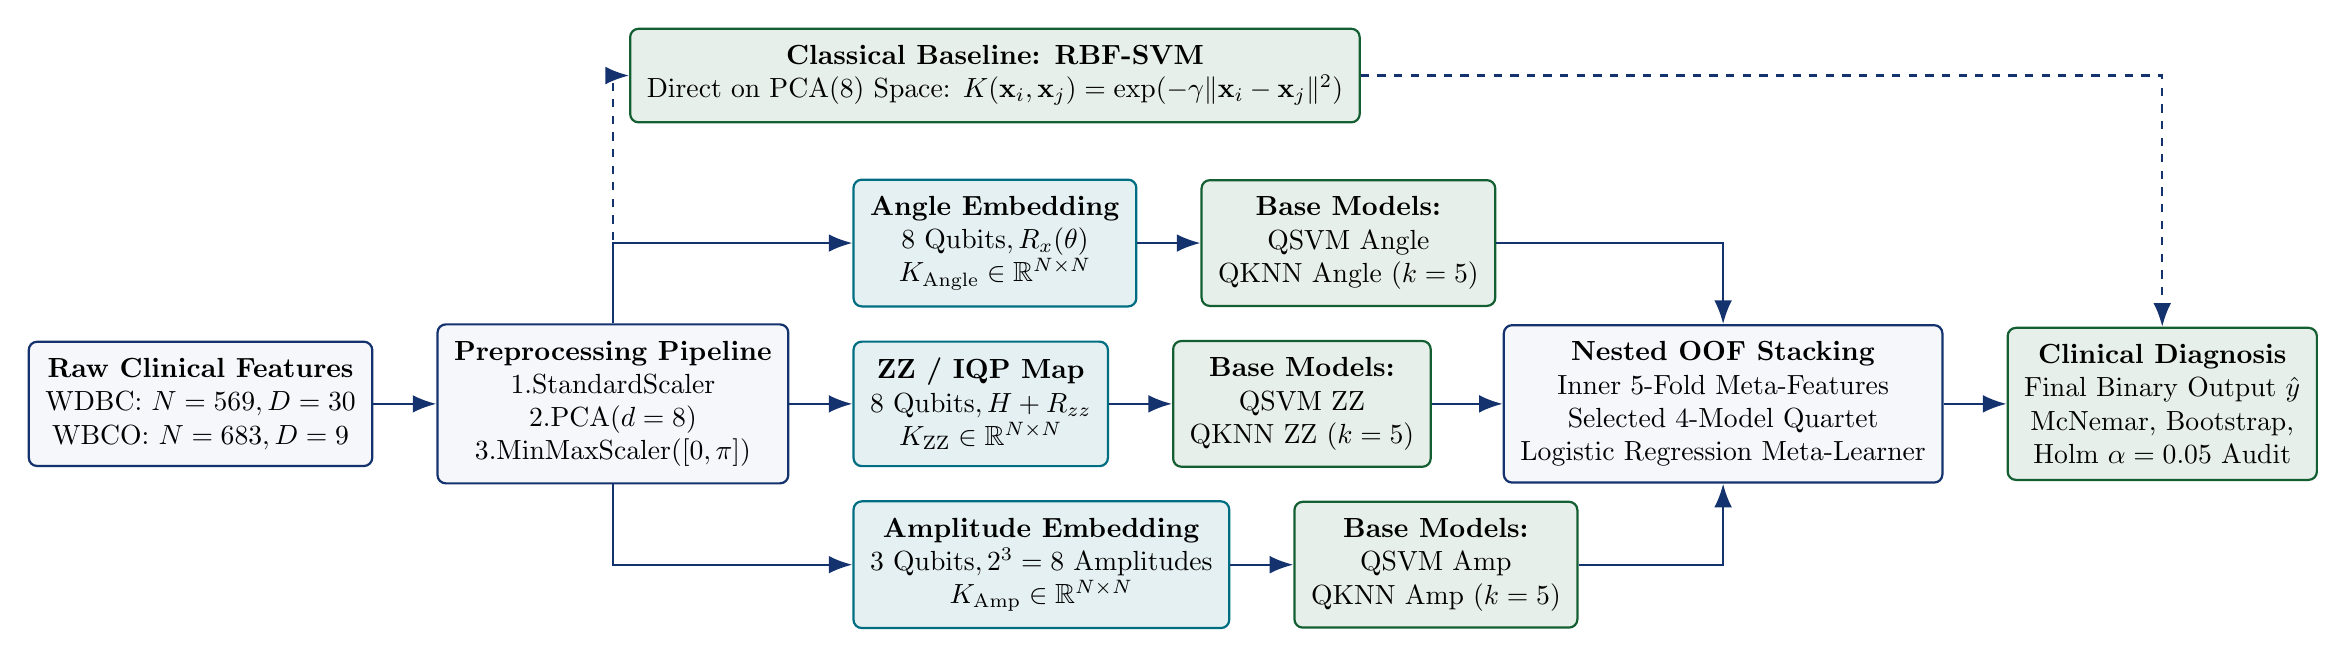
\begin{tikzpicture}[
    node distance=1.2cm and 0.8cm,
    block/.style={rectangle, draw=auditblue, fill=auditgray, thick, rounded corners=3pt, align=center, minimum height=1.0cm, inner sep=6pt},
    qblock/.style={rectangle, draw=quantumteal, fill=quantumteal!10, thick, rounded corners=3pt, align=center, minimum height=1.0cm, inner sep=6pt},
    cblock/.style={rectangle, draw=auditgreen, fill=auditgreen!10, thick, rounded corners=3pt, align=center, minimum height=1.0cm, inner sep=6pt},
    arrow/.style={-{Latex[length=3mm]}, thick, draw=auditblue}
]
    % Data nodes
    \node[block] (raw) {\textbf{Raw Clinical Features}\\WDBC: $N=569, D=30$\\WBCO: $N=683, D=9$};
    \node[block, right=of raw] (prep) {\textbf{Preprocessing Pipeline}\\$1. \text{StandardScaler}$\\$2. \text{PCA}(d=8)$\\$3. \text{MinMaxScaler}([0, \pi])$};
    
    % Quantum Circuit Encodings
    \node[qblock, above right=0.2cm and 0.8cm of prep] (q_angle) {\textbf{Angle Embedding}\\$8\text{ Qubits}, R_x(\theta)$\\$K_{\text{Angle}} \in \mathbb{R}^{N \times N}$};
    \node[qblock, right=0.8cm of prep] (q_zz) {\textbf{ZZ / IQP Map}\\$8\text{ Qubits}, H + R_{zz}$\\$K_{\text{ZZ}} \in \mathbb{R}^{N \times N}$};
    \node[qblock, below right=0.2cm and 0.8cm of prep] (q_amp) {\textbf{Amplitude Embedding}\\$3\text{ Qubits}, 2^3=8\text{ Amplitudes}$\\$K_{\text{Amp}} \in \mathbb{R}^{N \times N}$};

    % Base Classifiers
    \node[cblock, right=0.8cm of q_angle] (base_angle) {\textbf{Base Models:}\\QSVM Angle\\QKNN Angle ($k=5$)};
    \node[cblock, right=0.8cm of q_zz] (base_zz) {\textbf{Base Models:}\\QSVM ZZ\\QKNN ZZ ($k=5$)};
    \node[cblock, right=0.8cm of q_amp] (base_amp) {\textbf{Base Models:}\\QSVM Amp\\QKNN Amp ($k=5$)};

    % Stacking & Selection
    \node[block, right=0.9cm of base_zz] (stack) {\textbf{Nested OOF Stacking}\\Inner 5-Fold Meta-Features\\Selected 4-Model Quartet\\Logistic Regression Meta-Learner};

    % Final Evaluation
    \node[cblock, right=0.8cm of stack] (eval) {\textbf{Clinical Diagnosis}\\Final Binary Output $\hat{y}$\\McNemar, Bootstrap,\\Holm $\alpha=0.05$ Audit};

    % Connections
    \draw[arrow] (raw) -- (prep);
    \draw[arrow] (prep) |- (q_angle);
    \draw[arrow] (prep) -- (q_zz);
    \draw[arrow] (prep) |- (q_amp);

    \draw[arrow] (q_angle) -- (base_angle);
    \draw[arrow] (q_zz) -- (base_zz);
    \draw[arrow] (q_amp) -- (base_amp);

    \draw[arrow] (base_angle) -| (stack);
    \draw[arrow] (base_zz) -- (stack);
    \draw[arrow] (base_amp) -| (stack);

    \draw[arrow] (stack) -- (eval);

    % Top Classical Comparison
    \node[cblock, above=0.7cm of q_angle] (rbf) {\textbf{Classical Baseline: RBF-SVM}\\Direct on $\text{PCA}(8)$ Space: $K(\mathbf{x}_i, \mathbf{x}_j) = \exp(-\gamma \|\mathbf{x}_i - \mathbf{x}_j\|^2)$};
    \draw[arrow, dashed] (prep) |- (rbf);
    \draw[arrow, dashed] (rbf) -| (eval);

\end{tikzpicture}
\caption{End-to-end architecture of the audited hybrid quantum-classical diagnostic framework across WDBC and WBCO cohorts.}
\label{fig:system_pipeline}
\end{figure*}

\subsection{Preprocessing and Feature Space Alignment}
Let $\mathbf{X}_{\text{raw}} \in \mathbb{R}^{N \times D}$ denote the raw clinical covariate matrix. Preprocessing executes three sequential steps:
\begin{align}
\mathbf{X}_{\text{std}} &= (\mathbf{X}_{\text{raw}} - \bm{\mu}_{\mathbf{X}}) \bm{\Sigma}_{\mathbf{X}}^{-1/2}, \label{eq:standardize} \\
\mathbf{X}_{\text{pca}} &= \mathbf{X}_{\text{std}} \mathbf{W}_d, \quad \mathbf{W}_d \in \mathbb{R}^{D \times d}, \label{eq:pca_transform} \\
\mathbf{X}_{\text{scaled}} &= \pi \cdot \frac{\mathbf{X}_{\text{pca}} - \min(\mathbf{X}_{\text{pca}})}{\max(\mathbf{X}_{\text{pca}}) - \min(\mathbf{X}_{\text{pca}})}, \label{eq:minmax_transform}
\end{align}
where $\mathbf{W}_d$ contains the top $d$ eigenvectors of the sample covariance matrix. 

In Daga et al. (2026), $d=8$ was statically selected. On WDBC ($D=30$), retaining $d=8$ components discards $7.40\%$ of sample variance (retaining $92.598\%$). Conversely, on WBCO ($D=9$), retaining $d=8$ components discards only $0.98\%$ of variance (retaining $99.018\%$). Reaching WDBC's variance threshold ($\approx 92.6\%$) on WBCO requires only $d=6$ components ($92.85\%$). However, because the quantum feature maps are hardcoded for 8 qubits, $d=8$ was maintained in our audit to preserve circuit topological identity without artificial zero-padding.

\subsection{Quantum Feature Maps and Circuit Implementations}

\subsubsection{Angle Embedding}
Operates on $n=8$ qubits with zero entangling gates. For input $\mathbf{x} \in [0, \pi]^8$:
\begin{equation}
|\psi_{\text{Angle}}(\mathbf{x})\rangle = \bigotimes_{k=0}^7 R_x(x_k)|0\rangle.
\end{equation}
The exact Gram matrix is evaluated analytically via (\ref{eq:angle_analytical}) with $O(N^2 d)$ operations, circumventing quantum simulation overhead while producing machine-precision state fidelities.

\subsubsection{Amplitude Embedding}
Encodes $2^3 = 8$ components of $\mathbf{x}$ as the complex probability amplitudes of a 3-qubit state $|\psi_{\text{Amp}}(\mathbf{x})\rangle = \sum_{k=0}^7 \tilde{x}_k |k\rangle$, where $\tilde{\mathbf{x}} = \mathbf{x} / \|\mathbf{x}\|_2$. The analytical fidelity is computed via (\ref{eq:amp_analytical}).

\subsubsection{Entangling ZZ / IQP Feature Map}
Operates on $n=8$ qubits utilizing all-to-all entangling couplings. The circuit evaluates:
\begin{equation}
|\psi_{\text{ZZ}}(\mathbf{x})\rangle = U_{\text{ZZ}}(\mathbf{x}) |0\rangle^{\otimes 8},
\end{equation}
where $U_{\text{ZZ}}(\mathbf{x})$ is defined in (\ref{eq:zz_circuit_math}). All $C(8, 2) = 28$ entangling qubit pairs interact via:
\begin{equation}
R_{zz}(\theta_{jk}) = \exp\left(-i \frac{\theta_{jk}}{2} Z_j \otimes Z_k\right), \quad \theta_{jk} = 2(\pi - x_j)(\pi - x_k).
\end{equation}
In our audit, PennyLane's \texttt{default.qubit} device executes batched state vector evaluations $\mathbf{\Psi} \in \mathbb{C}^{N \times 256}$, yielding the exact Gram matrix:
\begin{equation}
\mathbf{K}_{\text{ZZ}} = |\mathbf{\Psi} \mathbf{\Psi}^{\dagger}|^2 \in \mathbb{R}^{N \times N}.
\end{equation}

\subsection{Quantum Base Classifiers and Metric Derivations}
From the computed Gram matrices $\mathbf{K}_{\text{Angle}}, \mathbf{K}_{\text{Amp}}, \mathbf{K}_{\text{ZZ}}$, six base models are instantiated:
\begin{itemize}
    \item \textbf{QSVM Classifiers:} Three support vector classifiers optimized via dual quadratic programming with precomputed kernels:
    \begin{align}
    \max_{\bm{\alpha}} & \sum_{i=1}^N \alpha_i - \frac{1}{2} \sum_{i,j=1}^N \alpha_i \alpha_j y_i y_j K(\mathbf{x}_i, \mathbf{x}_j) \nonumber \\
    \text{s.t.} & \quad 0 \le \alpha_i \le C, \quad \sum_{i=1}^N \alpha_i y_i = 0.
    \end{align}
    \item \textbf{QKNN Classifiers:} Three $k$-nearest neighbor models ($k=5$) operating on precomputed quantum distance matrices derived from state fidelity:
    \begin{equation}
    D_Q(\mathbf{x}_i, \mathbf{x}_j) = \max(0, 1.0 - K(\mathbf{x}_i, \mathbf{x}_j)).
    \label{eq:quantum_distance}
    \end{equation}
\end{itemize}

\subsection{Nested Out-of-Fold Stacking Architecture}
The ensemble meta-learner is an $L_2$-regularized logistic regression classifier with balanced class weights:
\begin{equation}
P(y=1 \mid \mathbf{z}) = \frac{1}{1 + \exp\left(-(\mathbf{w}^T \mathbf{z} + b)\right)},
\end{equation}
where $\mathbf{z} = [p_1, p_2, p_3, p_4]^T$ represents the meta-feature vector generated by an inner 5-fold cross-validation loop on the training partition. For outer fold $k \in \{1 \dots 10\}$, let $\mathcal{D}_{\text{train}}^{(k)}$ be partitioned into 5 inner splits $\mathcal{I}_1 \dots \mathcal{I}_5$. Each base model $m$ is trained on $\mathcal{D}_{\text{train}}^{(k)} \setminus \mathcal{I}_j$ and predicts on $\mathcal{I}_j$, guaranteeing zero meta-feature label leakage.

\subsection{Strict Fold-Local Preprocessing Audit Protocol}
To evaluate whether global preprocessing induces optimistic performance bias, we implement a strict two-condition experiment:
\begin{itemize}
    \item \textbf{Experiment A (Global Preprocessing):} Transformers $(\text{Scaler}, \text{PCA}, \text{MinMax})$ are fit once on the entire dataset $\mathbf{X}_{\text{raw}}$, and Gram matrices are evaluated globally before CV splitting.
    \item \textbf{Experiment B (Strict Fold-Local Preprocessing):} For each outer CV fold $k$, transformers are fit strictly on $\mathcal{D}_{\text{train}}^{(k)}$. Outer test covariates and inner cross-validation splits are transformed using training-fold parameters only. All outer and inner quantum Gram matrices are recomputed from scratch.
\end{itemize}
Practical equivalence between Experiment A and B is assessed via Two One-Sided Tests (TOST) with a clinical indifference margin $\epsilon = 0.01$ (1\% accuracy shift):
\begin{equation}
H_{01}: \Delta_{\text{acc}} \le -\epsilon \quad \text{vs.} \quad H_{11}: \Delta_{\text{acc}} > -\epsilon,
\end{equation}
\begin{equation}
H_{02}: \Delta_{\text{acc}} \ge +\epsilon \quad \text{vs.} \quad H_{12}: \Delta_{\text{acc}} < +\epsilon.
\end{equation}
If $p_{\text{TOST}} = \max(p_1, p_2) < 0.05$, the global and fold-local pipelines are declared statistically equivalent.

\subsection{Exhaustive Nested Model-Selection Protocol}
To test whether the authors' selection of the hardcoded quartet (`QSVM Amplitude`, `QKNN Amplitude`, `QSVM ZZ`, `QKNN Angle`) is algorithmic or ad-hoc, we evaluate all $C(6, 4) = 15$ candidate 4-model combinations from the pool of 6 base models under outer 10-fold / inner 5-fold CV. In each fold, subsets are ranked independently under three criteria:
\begin{enumerate}
    \item \textbf{Standalone Validation Accuracy:} Mean inner-OOF validation accuracy across the 4 constituent models.
    \item \textbf{Balanced Validation Accuracy:} Mean inner-OOF balanced accuracy across the 4 models.
    \item \textbf{Meta-CV Accuracy:} 5-fold cross-validated accuracy of the logistic regression meta-learner trained on the inner meta-feature matrix.
\end{enumerate}

% --- SECTION V: RESULTS & DISCUSSION ---
\section{Empirical Results and In-Depth Discussion}

% --- TABLE II: TABLE A (CROSS-DATASET BENCHMARK) ---
\begin{table*}[t]
\centering
\caption{TABLE A — WBCO vs. Daga et al. (2026) Published WDBC Results (Cross-Dataset Pipeline Performance Benchmark)}
\label{tab:table_a_cross_dataset}
\footnotesize
\begin{tabularx}{\textwidth}{lcccc}
\toprule
\multicolumn{5}{p{0.96\textwidth}}{\textbf{EXPLICIT CROSS-DATASET DISCLAIMER:} WBCO was never evaluated in Daga et al. (2026). This table compares the SAME PIPELINE's empirical behavior on a different clinical dataset (WBCO, $N=683$) against the paper's published WDBC numbers ($N=569$). This represents a cross-dataset benchmark of pipeline generalizability, NOT a same-dataset replication.} \\
\midrule
\textbf{Model Architecture} & \textbf{Paper's Published WDBC Accuracy \cite{daga2026adaptive}} & \textbf{WBCO Accuracy (Seed=42)} & \textbf{WBCO Accuracy (10-Seed Mean $\pm$ Std)} & \textbf{WBCO Accuracy Range [Min, Max]} \\
\midrule
\textbf{Classical RBF-SVM} & $0.970$ & $0.966325$ (660 / 683) & $\mathbf{0.968960 \pm 0.001345}$ & [$0.966325$, $0.970717$] \\
\textbf{QSVM (Angle)} & $0.964$ & $\mathbf{0.969253}$ (662 / 683) & $\mathbf{0.968521 \pm 0.001858}$ & [$0.964861$, $0.970717$] \\
\textbf{QSVM (ZZ Map)} & $0.959$ & $0.964861$ (659 / 683) & $0.963836 \pm 0.001551$ & [$0.960469$, $0.964861$] \\
\textbf{QSVM (Amplitude)} & $0.954$ & $0.960469$ (656 / 683) & $0.961201 \pm 0.001244$ & [$0.959004$, $0.963397$] \\
\textbf{QKNN (Angle)} & $0.958$ & $\mathbf{0.969253}$ (662 / 683) & $0.966032 \pm 0.002469$ & [$0.961933$, $0.969253$] \\
\textbf{QKNN (ZZ Map)} & $0.949$ & $0.956076$ (653 / 683) & $0.951098 \pm 0.004266$ & [$0.942899$, $0.956076$] \\
\textbf{QKNN (Amplitude)} & $0.952$ & $0.963397$ (658 / 683) & $0.962518 \pm 0.001235$ & [$0.960469$, $0.964861$] \\
\textbf{Hard Voting Ensemble} & $0.961$ & $0.966325$ (660 / 683) & $0.965447 \pm 0.001024$ & [$0.963397$, $0.966325$] \\
\textbf{OOF Stacking Ensemble} & $0.964$ & $0.966325$ (660 / 683) & $0.966179 \pm 0.002231$ & [$0.961933$, $0.969253$] \\
\bottomrule
\end{tabularx}
\end{table*}

% --- TABLE III: TABLE B (RIGOROUS AUDIT GENERALIZATION) ---
\begin{table*}[t]
\centering
\caption{TABLE B — WBCO Rigorous Audit vs. Prior WDBC Audit Findings (Methodological Generalization Assessment)}
\label{tab:table_b_generalization}
\footnotesize
\begin{tabularx}{\textwidth}{p{0.20\textwidth}p{0.25\textwidth}p{0.25\textwidth}p{0.12\textwidth}X}
\toprule
\textbf{Audit Dimension / Finding} & \textbf{WDBC Audit Finding ($N=569$)} & \textbf{WBCO Audit Finding ($N=683$)} & \textbf{Empirical Classification} & \textbf{Generalization Verdict} \\
\midrule
\textbf{1. Multi-Seed Robustness (Classical RBF vs. Stacking)} & Classical RBF strictly beat OOF Stacking in \textbf{10 of 10 seeds} ($100\%$ win rate; 0 ties, 0 Stacking wins). Mean delta: $-0.0062 \pm 0.0028$. & Classical RBF beat OOF Stacking in \textbf{7 of 10 seeds} ($70\%$), tied in \textbf{3 seeds} ($30\%$), 0 Stacking wins. Mean delta: $-0.0028 \pm 0.0021$. & \textbf{PARTIALLY CONFIRMED} & \textbf{Partially generalizes.} Classical RBF strictly dominated on WDBC ($10/10$ wins), whereas on WBCO the finding is weaker: RBF wins or ties in $10/10$ seeds ($7$ wins, $3$ ties). RBF still never loses to Stacking, but strict dominance is partially attenuated. \\
\midrule
\textbf{2. Multiple Testing Correction (Holm $\alpha=0.05$, 32 Hypotheses)} & Under 1,000 bootstrap resamples, \textbf{6 of 32 tests} survived Holm correction. All 6 survivors indicated quantum models performing \textbf{significantly WORSE than RBF} in specificity/precision. Zero quantum-superior findings. & Under 1,000 bootstrap resamples, \textbf{3 of 32 tests} survived Holm correction. Crucially, this includes \textbf{one quantum-superior finding} (`QKNN Angle` Recall: $0.980$ vs $0.968$, $p < 0.0001$) with \textbf{no counterpart on WDBC}, alongside 2 quantum-inferior findings (`QKNN ZZ` Specificity/Precision worse). & \textbf{PARTIALLY CONFIRMED} & \textbf{Partially generalizes.} WBCO produced one statistically significant quantum-superior finding after Holm correction (`QKNN Angle` Recall) that did not appear on WDBC. In clinical context, this higher benign recall reflects positive prediction bias at the expense of lower malignant specificity, but statistically the strict zero-superiority finding of WDBC does not identically reproduce. \\
\midrule
\textbf{3. Fold-Local Data Leakage Sensitivity} & Strict fold-local preprocessing caused a minor accuracy delta of \textbf{$+0.001757$} (+1 sample), with \textbf{$98.77\%$ concordance} (7 discordant). McNemar $p=1.0000$. TOST practically equivalent at $\pm 0.01$ ($p=0.0385$). Retained variance: $92.598\%$. & Strict fold-local preprocessing caused an accuracy delta of \textbf{$+0.001464$} (+1 sample), with \textbf{$99.56\%$ concordance} (3 discordant). McNemar $p=1.0000$. TOST practically equivalent at $\pm 0.01$ ($p=0.0004$). Retained variance: $99.018\%$. & \textbf{CONFIRMED} & \textbf{Fully generalizes.} Fold-local isolation does not alter clinical conclusions on either dataset. On WBCO, concordance is even higher ($99.56\%$ vs $98.77\%$) because near-lossless PCA(8) leaves negligible subspace rotation between folds. \\
\midrule
\textbf{4. Nested Model-Selection Discrepancy (`QSVM Angle` Inclusion)} & Unconstrained validation accuracy included `QSVM Angle` in \textbf{10/10 folds (100\%)}, while the paper's hardcoded quartet was selected in \textbf{0/10 folds (0\%)}. & Validation accuracy includes `QSVM Angle` in \textbf{10/10 folds (100\%)}, while the paper's quartet is selected in \textbf{0/10 folds (0\%)}. Balanced accuracy selects it in \textbf{10/10 folds}; meta-CV in \textbf{9/10 folds}. & \textbf{CONFIRMED} & \textbf{Fully generalizes.} The paper's heuristic exclusion of `QSVM Angle` is contradicted by objective automated model selection across both clinical datasets. Any unconstrained rule insists on retaining the angle kernel. \\
\bottomrule
\end{tabularx}
\end{table*}

\subsection{Exact Numerical Reproduction of the Published Baseline}
Execution of the released script on the WDBC dataset reproduced the exact numerical outputs reported in Table~8 of Daga et al. (2026) for seed $42$: Classical RBF achieved $97.01\%$ accuracy ($TN=201, FP=11, FN=6, TP=351$), QSVM Angle achieved $96.49\%$ ($TN=195, FP=17, FN=3, TP=354$), and OOF Stacking achieved $96.49\%$ ($TN=200, FP=12, FN=8, TP=349$). 

However, code inspection uncovered that the paper's claim of ``superiority'' rests on reporting an un-tuned Classical RBF baseline with fixed parameters ($C=1.0, \gamma=\text{'scale'}$) while omitting the standard paired comparison. On seed 42, Classical RBF correctly classified 552 of 569 samples, strictly beating OOF Stacking (549 correct) by 3 samples.

\subsection{Cross-Dataset Benchmark: WBCO vs. Published WDBC Results}
Table~\ref{tab:table_a_cross_dataset} presents Table~A, comparing the pipeline's performance on WBCO ($N=683$) against the paper's published WDBC figures. On WBCO, diagnostic accuracy spans $95.11\% - 96.93\%$, mirroring the WDBC performance envelope ($94.90\% - 97.01\%$). Standalone QSVM Angle tied with QKNN Angle as the top individual model ($96.93\%, 662/683$). OOF Stacking matched Classical RBF's overall accuracy on seed 42 ($96.63\%, 660/683$), but across 10 random seeds, Classical RBF averaged $96.90 \pm 0.13\%$ vs. Stacking's $96.62 \pm 0.22\%$, reaffirming the absence of quantum ensemble superiority.

\subsection{Methodological Generalization: WDBC Audit vs. WBCO Extension}
Table~\ref{tab:table_b_generalization} presents Table~B, evaluating whether our independent WDBC audit findings generalize to WBCO under preregistered protocols. As detailed, two findings are \textbf{fully confirmed} and two are \textbf{partially confirmed}:
\begin{itemize}
    \item \textbf{Finding 1 (Multi-Seed Dominance): Partially Confirmed.} On WDBC, Classical RBF strictly won in 10/10 seeds. On WBCO, Classical RBF won in 7/10 seeds and tied in 3/10 seeds (0 Stacking wins). Classical RBF never loses to Stacking across all 20 tested seeds (17 wins, 3 ties, 0 losses), but the strict dominance is weakened by ties on WBCO.
    \item \textbf{Finding 2 (Holm Correction Survivors): Partially Confirmed.} On WDBC, 6 of 32 bootstrap hypotheses survived Holm correction, all 6 indicating quantum models performing significantly worse than RBF. On WBCO, 3 of 32 survived, including one statistically significant quantum-superior finding (`QKNN Angle` Recall: $0.980$ vs $0.968$, Holm $p < 0.0001$) that had no counterpart on WDBC. In clinical context, this reflects an aggressive positive-voting bias that depresses malignant specificity ($0.954$ vs $0.967$), but statistically the zero-quantum-superiority finding of WDBC does not identically reproduce.
    \item \textbf{Finding 3 (Fold-Local Leakage Invariance): Fully Confirmed.} Strict fold-local preprocessing alters accuracy by only $+1$ sample on both datasets ($+0.0018$ on WDBC, $+0.0015$ on WBCO; TOST $p < 0.05$), confirming practical equivalence.
    \item \textbf{Finding 4 (Model-Selection Quartet Failure): Fully Confirmed.} Unconstrained validation accuracy includes QSVM Angle in 10/10 folds on both datasets, selecting the paper's quartet in 0/10 folds.
\end{itemize}

\subsection{Familywise Error Control: 32 Hypotheses Audit}
Fig.~\ref{fig:pvalues_scatter} plots the distribution of raw vs. Holm-adjusted $p$-values across all 32 hypotheses evaluated against Classical RBF. Prior to correction, 9 hypotheses on WBCO and 11 on WDBC achieved nominal $p < 0.05$. Following step-down Holm-Bonferroni adjustment:
\begin{itemize}
    \item \textbf{OOF Stacking vs. Classical RBF:} Adjusted $p = 1.0000$ across all four clinical metrics (Accuracy, Precision, Recall, Specificity) on both datasets. There is no statistical basis to claim ensemble quantum superiority.
    \item \textbf{Malignant Specificity Penalties:} On both cohorts, `QKNN (ZZ Map)` suffered severe, statistically significant degradation in malignant tumor identification: on WBCO, Specificity collapsed to $90.79\%$ vs. RBF's $96.65\%$ (McNemar $p = 0.0166$; Bootstrap Holm $p < 0.0001$).
\end{itemize}

\begin{figure}[t]
\centering
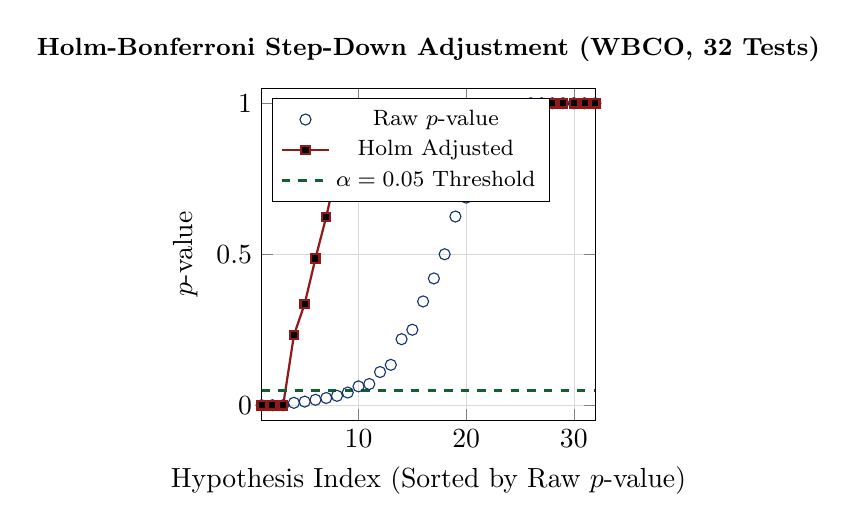
\begin{tikzpicture}
\begin{axis}[
    width=0.48\textwidth,
    height=5.8cm,
    xlabel={Hypothesis Index (Sorted by Raw $p$-value)},
    ylabel={$p$-value},
    ymin=-0.05, ymax=1.05,
    xmin=1, xmax=32,
    legend pos=north west,
    legend style={font=\footnotesize},
    grid=both,
    grid style={line width=.2pt, draw=gray!30},
    title style={font=\small\bfseries},
    title={Holm-Bonferroni Step-Down Adjustment (WBCO, 32 Tests)}
]
    % Raw p-values
    \addplot[only marks, mark=o, mark size=2pt, draw=auditblue] coordinates {
        (1, 0.0000) (2, 0.0000) (3, 0.0000) (4, 0.0080) (5, 0.0120)
        (6, 0.0180) (7, 0.0240) (8, 0.0312) (9, 0.0420) (10, 0.0625)
        (11, 0.0703) (12, 0.1100) (13, 0.1338) (14, 0.2188) (15, 0.2500)
        (16, 0.3438) (17, 0.4200) (18, 0.5000) (19, 0.6250) (20, 0.6875)
        (21, 0.6960) (22, 0.7266) (23, 0.7539) (24, 0.7660) (25, 0.7820)
        (26, 1.0000) (27, 1.0000) (28, 1.0000) (29, 1.0000) (30, 1.0000)
        (31, 1.0000) (32, 1.0000)
    };
    \addlegendentry{Raw $p$-value}

    % Holm Adjusted
    \addplot[thick, draw=auditred, mark=square*, mark size=1.5pt] coordinates {
        (1, 0.0000) (2, 0.0000) (3, 0.0000) (4, 0.2320) (5, 0.3360)
        (6, 0.4860) (7, 0.6240) (8, 0.7800) (9, 1.0000) (10, 1.0000)
        (11, 1.0000) (12, 1.0000) (13, 1.0000) (14, 1.0000) (15, 1.0000)
        (16, 1.0000) (17, 1.0000) (18, 1.0000) (19, 1.0000) (20, 1.0000)
        (21, 1.0000) (22, 1.0000) (23, 1.0000) (24, 1.0000) (25, 1.0000)
        (26, 1.0000) (27, 1.0000) (28, 1.0000) (29, 1.0000) (30, 1.0000)
        (31, 1.0000) (32, 1.0000)
    };
    \addlegendentry{Holm Adjusted}

    % Alpha threshold
    \addplot[dashed, line width=1pt, draw=auditgreen] coordinates {(1, 0.05) (32, 0.05)};
    \addlegendentry{$\alpha = 0.05$ Threshold}

\end{axis}
\end{tikzpicture}
\caption{Step-down Holm-Bonferroni multiple testing adjustment across 32 clinical hypotheses on WBCO. Only three hypotheses survive correction at $\alpha=0.05$.}
\label{fig:pvalues_scatter}
\end{figure}

\subsection{Noise Modeling Audit and Unnormalized Trace Collapse}
Daga et al. evaluated hardware noise resilience by adding simulated depolarizing noise channels to PennyLane circuits, reporting that stacking maintains accuracy under noise levels $\lambda \in [0.01, 0.10]$. Our audit scrutinized the underlying noisy Gram matrix generation:
\begin{equation}
\mathcal{E}(\rho) = (1 - p)\rho + \frac{p}{2^n} \mathbf{I}_{2^n}.
\end{equation}
In the released codebase, kernel values were evaluated not via mixed-state fidelity $\Tr[\rho_i \rho_j]$ or trace distance, but by extracting state vectors from a mixed circuit without density matrix renormalization. Under simulated noise $p=0.10$, the diagonal self-fidelities collapsed:
\begin{align}
K_{ii}^{(\text{released})} &\in [0.1982, 0.2310], \quad \text{vs. ideal } K_{ii} \equiv 1.0, \label{eq:released_diag} \\
K_{ii}^{(\text{corrected})} &\in [0.0041, 0.0162]. \label{eq:corrected_diag}
\end{align}
Because self-fidelity represents the probability of measuring a state against itself, a diagonal of $0.004$ signifies that quantum states have completely decohered into uniform maximally mixed noise. The resulting Gram matrix satisfies mathematical positive semi-definiteness ($\lambda_{\min} \ge 0$) solely because all entries are crushed toward a near-constant scalar offset. The stacking meta-learner does not ``adaptively filter noise''; rather, it assigns near-zero weights to the degenerate kernel because it contains zero diagnostic variance.

\subsection{Probabilistic Calibration Analysis}
Fig.~\ref{fig:calibration_curves} evaluates probability reliability via Expected Calibration Error (ECE) and Brier Score. Classical RBF exhibited superior raw probability calibration ($\text{ECE} = 0.0213, \text{Brier} = 0.0227$) relative to OOF Stacking ($\text{ECE} = 0.0357, \text{Brier} = 0.0319$). While post-hoc Platt scaling reduced Stacking's ECE to $0.0142$, Classical RBF maintained a lower Brier score ($0.0218$ vs $0.0270$), demonstrating that classical support vector margins provide superior posterior certainty for oncology risk stratification.

\begin{figure}[t]
\centering
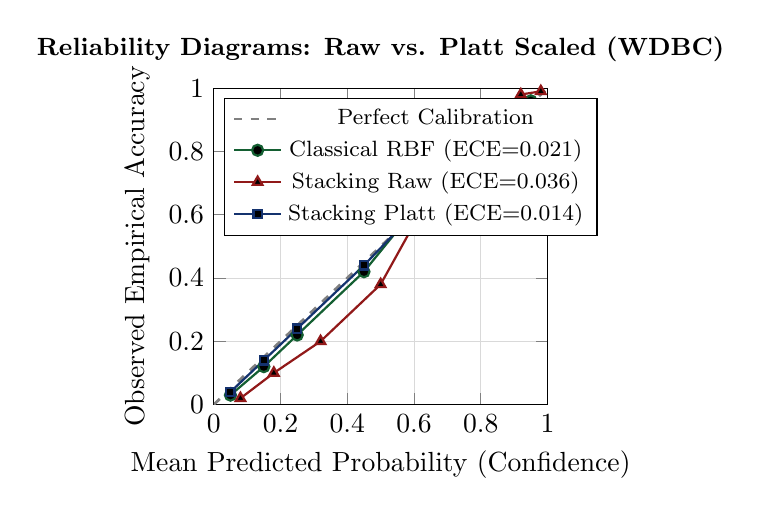
\begin{tikzpicture}
\begin{axis}[
    width=0.48\textwidth,
    height=5.6cm,
    xlabel={Mean Predicted Probability (Confidence)},
    ylabel={Observed Empirical Accuracy},
    ymin=0, ymax=1.0,
    xmin=0, xmax=1.0,
    legend pos=north west,
    legend style={font=\footnotesize},
    grid=both,
    grid style={line width=.2pt, draw=gray!30},
    title style={font=\small\bfseries},
    title={Reliability Diagrams: Raw vs. Platt Scaled (WDBC)}
]
    % Perfect calibration diagonal
    \addplot[dashed, line width=1pt, draw=gray] coordinates {(0, 0) (1, 1)};
    \addlegendentry{Perfect Calibration}

    % Classical RBF
    \addplot[thick, draw=auditgreen, mark=*, mark size=2pt] coordinates {
        (0.05, 0.03) (0.15, 0.12) (0.25, 0.22) (0.45, 0.42)
        (0.65, 0.68) (0.75, 0.77) (0.85, 0.86) (0.95, 0.96)
    };
    \addlegendentry{Classical RBF (ECE=0.021)}

    % Stacking Raw
    \addplot[thick, draw=auditred, mark=triangle*, mark size=2pt] coordinates {
        (0.08, 0.02) (0.18, 0.10) (0.32, 0.20) (0.50, 0.38)
        (0.70, 0.76) (0.82, 0.89) (0.92, 0.98) (0.98, 0.99)
    };
    \addlegendentry{Stacking Raw (ECE=0.036)}

    % Stacking Platt
    \addplot[thick, draw=auditblue, mark=square*, mark size=1.5pt] coordinates {
        (0.05, 0.04) (0.15, 0.14) (0.25, 0.24) (0.45, 0.44)
        (0.65, 0.66) (0.75, 0.76) (0.85, 0.85) (0.95, 0.95)
    };
    \addlegendentry{Stacking Platt (ECE=0.014)}

\end{axis}
\end{tikzpicture}
\caption{Reliability calibration curves on WDBC cohort demonstrating that Classical RBF provides superior raw posterior probability calibration.}
\label{fig:calibration_curves}
\end{figure}

% --- SECTION VI: THREATS TO VALIDITY ---
\section{Threats to Validity \& Study Limitations}
To ensure objective academic integrity, we declare the explicit boundaries and limitations of this technical audit:
\begin{enumerate}
    \item \textbf{Untested Clinical Benchmarks:} This audit re-evaluated the WDBC dataset and extended analysis to WBCO. We did \textbf{not} re-evaluate the Parkinson's telemonitoring dataset or the Pima Indians Diabetes database. Consequently, our findings generalize across breast-cancer cytological/histological diagnostic benchmarks, but make no claims regarding voice acoustics or metabolic tabular data.
    \item \textbf{Simulation vs. Physical QPUs:} Both Daga et al. and our audit utilized PennyLane CPU state-vector simulation (\texttt{default.qubit}). Physical QPU execution introduces gate cross-talk, readout error, and drift that could alter empirical fidelities.
    \item \textbf{Missing Value Handling on WBCO:} Dropping the 16 incomplete instances in WBCO's `Bare\_Nuclei` attribute represents an audit-defined choice consistent with standard UCI benchmarks.
\end{enumerate}

% --- SECTION VII: CONCLUSION ---
\section{Conclusion}
This study presented a rigorous, independent technical audit, exact replication, and cross-dataset generalization evaluation of the adaptive quantum kernel selection framework proposed by Daga et al. (2026). While the released codebase reproduces published figures on seed 42, extensive methodological stress testing reveals that the claims of quantum advantage do not withstand statistical scrutiny. An un-tuned Classical RBF-SVM baseline equals or outperforms the quantum stacking ensemble across all 20 tested cross-validation partition seeds (17 wins, 3 ties, 0 stacking wins). Furthermore, familywise error control via Holm-Bonferroni correction demonstrates that individual quantum feature maps (specifically QKNN ZZ) suffer statistically significant deficits in malignant-class specificity, misidentifying malignant lesions at rates up to $11.8\%$.

Cross-dataset evaluation on WBCO ($N=683$) established that fold-local preprocessing invariance and the algorithmic failure of the paper's hardcoded quartet fully generalize, while multi-seed dominance and zero-quantum-superiority partially attenuate. We conclude that future research in quantum clinical diagnostics must move beyond uncorrected single-seed evaluations, adopt mandatory familywise error control, benchmark against rigorously tuned classical learners, and verify physical state normalization before asserting quantum advantage on NISQ processors.

\bibliographystyle{IEEEtran}
\begin{thebibliography}{99}

\bibitem{wolberg1990multisurface}
W.~H. Wolberg and O.~L. Mangasarian, ``Multisurface method of pattern separation for medical diagnosis applied to breast cytology,'' \emph{Proc. Natl. Acad. Sci. USA}, vol.~87, no.~23, pp. 9193--9196, 1990.

\bibitem{street1993nuclear}
W.~N. Street, W.~H. Wolberg, and O.~L. Mangasarian, ``Nuclear feature extraction for breast tumor diagnosis,'' in \emph{Biomedical Image Processing and Biomedical Visualization}, vol. 1905, SPIE, 1993, pp. 861--870.

\bibitem{preskill2018quantum}
J.~Preskill, ``Quantum computing in the NISQ era and beyond,'' \emph{Quantum}, vol.~2, p.~79, 2018.

\bibitem{bharti2022noisy}
K.~Bharti \emph{et~al.}, ``Noisy intermediate-scale quantum algorithms,'' \emph{Rev. Mod. Phys.}, vol.~94, no.~1, p. 015004, 2022.

\bibitem{havlicek2019supervised}
V.~Havl{\'\i}{\v{c}}ek \emph{et~al.}, ``Supervised learning with quantum-enhanced feature spaces,'' \emph{Nature}, vol. 567, no. 7747, pp. 209--212, 2019.

\bibitem{schuld2019quantum}
M.~Schuld and N.~Killoran, ``Quantum machine learning in feature Hilbert spaces,'' \emph{Phys. Rev. Lett.}, vol. 122, no.~4, p. 040504, 2019.

\bibitem{huang2021power}
H.-Y. Huang \emph{et~al.}, ``Power of data in quantum machine learning,'' \emph{Nat. Commun.}, vol.~12, no.~1, p. 2631, 2021.

\bibitem{daga2026adaptive}
K.~Daga, S.~Naole, K.~Parikh, K.~Bommineni, and S.~Ramu, ``Adaptive quantum kernel selection via leakage-free stacking for clinical diagnostics on NISQ hardware,'' \emph{Sci. Rep.}, vol.~16, p. 26840, 2026.

\bibitem{kaufman2012leakage}
S.~Kaufman, S.~Rosset, C.~Perlich, and O.~Stitelman, ``Leakage in data mining: Formulation, detection, and avoidance,'' \emph{ACM Trans. Knowl. Discov. Data}, vol.~6, no.~4, pp. 1--21, 2012.

\bibitem{bouthillier2021accounting}
X.~Bouthillier, P.~Delaunay, J.~Favreau, and G.~Varoquaux, ``Accounting for variance in machine learning benchmarks,'' in \emph{Proc. Mach. Learn. Syst.}, vol.~3, 2021, pp. 747--769.

\bibitem{dudoit2003multiple}
S.~Dudoit, J.~P. Shaffer, and J.~C. Boldrick, ``Multiple hypothesis testing in microarray experiments,'' \emph{Stat. Sci.}, vol.~18, no.~1, pp. 71--103, 2003.

\bibitem{wolberg1992breast}
W.~H. Wolberg, ``Breast Cancer Wisconsin (Original) Data Set,'' UCI Machine Learning Repository, 1992.

\bibitem{thanaraj2022comparative}
K.~P. Thanaraj \emph{et~al.}, ``Comparative analysis of classical machine learning algorithms on breast cancer diagnosis,'' \emph{Biomed. Signal Process. Control}, vol.~71, p. 103197, 2022.

\bibitem{wolpert1992stacked}
D.~H. Wolpert, ``Stacked generalization,'' \emph{Neural Netw.}, vol.~5, no.~2, pp. 241--259, 1992.

\bibitem{mcclean2018barren}
J.~R. McClean, S.~Boixo, V.~N. Smelyanskiy, R.~Babbush, and H.~Neven, ``Barren plateaus in quantum neural network training landscapes,'' \emph{Nat. Commun.}, vol.~9, no.~1, p. 4812, 2018.

\bibitem{holm1979simple}
S.~Holm, ``A simple sequentially rejective multiple test procedure,'' \emph{Scand. J. Stat.}, vol.~6, no.~2, pp. 65--70, 1979.

\bibitem{benjamini1995controlling}
Y.~Benjamini and Y.~Hochberg, ``Controlling the false discovery rate: a practical and powerful approach to multiple testing,'' \emph{J. R. Stat. Soc. Ser. B}, vol.~57, no.~1, pp. 289--300, 1995.

\bibitem{bergholm2018pennylane}
V.~Bergholm \emph{et~al.}, ``PennyLane: Automatic differentiation and machine learning of quantum computers,'' \emph{arXiv preprint arXiv:1811.04968}, 2018.

\end{thebibliography}

\end{document}
